\documentclass[../../main.tex]{subfiles}

\graphicspath{{../../image/}{../../figure/}}

\begin{document}

\section{学习曲线}\label{section:ch09-学习曲线}

我们已经探讨了模型的泛化能力如何随模型中参数的数量、数据集的大小以及权重衰减正则化项的系数而变化。这些都允许我们在偏差和方差之间进行权衡，以最小化泛化误差。另一个影响这种权衡的因素是学习过程本身。在通过梯度下降优化误差函数期间，训练误差通常随着模型参数的更新而降低，而留出数据（hold-out data）的误差可能是非单调的。这种现象可以通过使用学习曲线来可视化。学习曲线显示了在迭代式学习过程（如随机梯度下降）中，性能指标（如训练集和验证集误差）关于迭代次数的变化。学习曲线不仅提供了对训练进程的洞察，还提供了一种控制模型有效复杂度的实用方法。

\begin{definition}[学习曲线]\label{definition:ch09-学习曲线}
设模型由迭代式优化算法训练，$\tau=0,1,2,\cdots$ 为迭代次数（或训练轮次）。称函数
\begin{align*}
\tau\mapsto\bigl(E_{\mathrm{train}}(\tau),E_{\mathrm{val}}(\tau)\bigr)
\end{align*}
为\textbf{学习曲线}（learning curve），其中 $E_{\mathrm{train}}(\tau)$ 与 $E_{\mathrm{val}}(\tau)$ 分别是第 $\tau$ 步时在训练集与验证集（留出数据）上计算的误差。若横轴改为训练集大小 $N$，相应的曲线称为\textbf{样本量学习曲线}。
\end{definition}

% SUPPLEMENT: parent=definition:ch09-学习曲线; kind=motivation; location=紧随其后的 remark（重构新增）
\begin{remark}（重构新增）\cref{definition:ch09-学习曲线}把“训练过程”本身当作一个可调节模型复杂度的维度：固定模型容量而改变训练多久，等价于在“欠拟合—过拟合”之间移动。这与调 $\lambda$、调参数个数是三种不同的复杂度控制方式，但它们在偏差--方差意义下有相似的效应。读学习曲线时要注意两点：验证误差的非单调性是过拟合的直接信号，但它的最小值位置依赖验证集的大小与划分，因此早停的轮次本身是一个需要估计的超参数；训练误差通常单调下降，若它下降而验证误差同时上升，说明模型开始记忆训练集中的噪声，而不是学到了可迁移的结构。
\end{remark}

\subsection{早停法}\label{subsection:ch09-早停法}

除正则化外，控制网络有效复杂度的一种替代方法是\textbf{早停法}（early stopping）。深度学习模型的训练涉及迭代下降定义在一组训练数据上的误差函数。虽然在训练集上计算的误差大致上关于迭代次数单调递减，但在留出数据（通常称为验证集）上计算的误差通常首先下降，然后由于网络开始过拟合而增加。因此，为了获得具有良好泛化能力的网络，应在验证集上的最小误差点处停止训练，如\cref{figure:ch09-学习曲线}所示。

\begin{definition}[早停法]\label{definition:ch09-早停法}
设 $\{\boldsymbol{w}^{(\tau)}\}_{\tau\geqslant0}$ 是迭代训练产生的参数序列，$E_{\mathrm{val}}(\tau)$ 为相应的验证误差。若训练在
\begin{align*}
\tau^{\star}\in\arg\min_{\tau\geqslant0}E_{\mathrm{val}}(\tau)
\end{align*}
处停止，并以 $\boldsymbol{w}^{(\tau^{\star})}$ 作为最终模型，则称这一训练策略为\textbf{早停法}（early stopping）。$\tau^{\star}$ 称为\textbf{停止轮次}。
\end{definition}

% SUPPLEMENT: parent=definition:ch09-早停法; kind=motivation; location=紧随其后的 remark（重构新增）
\begin{remark}（重构新增）\cref{definition:ch09-早停法}看起来只是“提前结束训练”，但它实质上是一种正则化：它限制了参数从初始化点出发所能走过的距离，从而限制了模型的有效复杂度。与权重衰减不同，早停几乎不增加计算成本（本来就要监控验证误差），也不需要修改误差函数；代价是它引入了新的超参数 $\tau^{\star}$，而且这个超参数依赖验证集的划分。还需注意，$\arg\min$ 可能不唯一，实践中通常取第一个达到最小值的轮次，并在其附近做平滑或 patience 机制，以避免验证误差的随机波动导致过早停止。
\end{remark}

\begin{figure}[htbp]
\centering
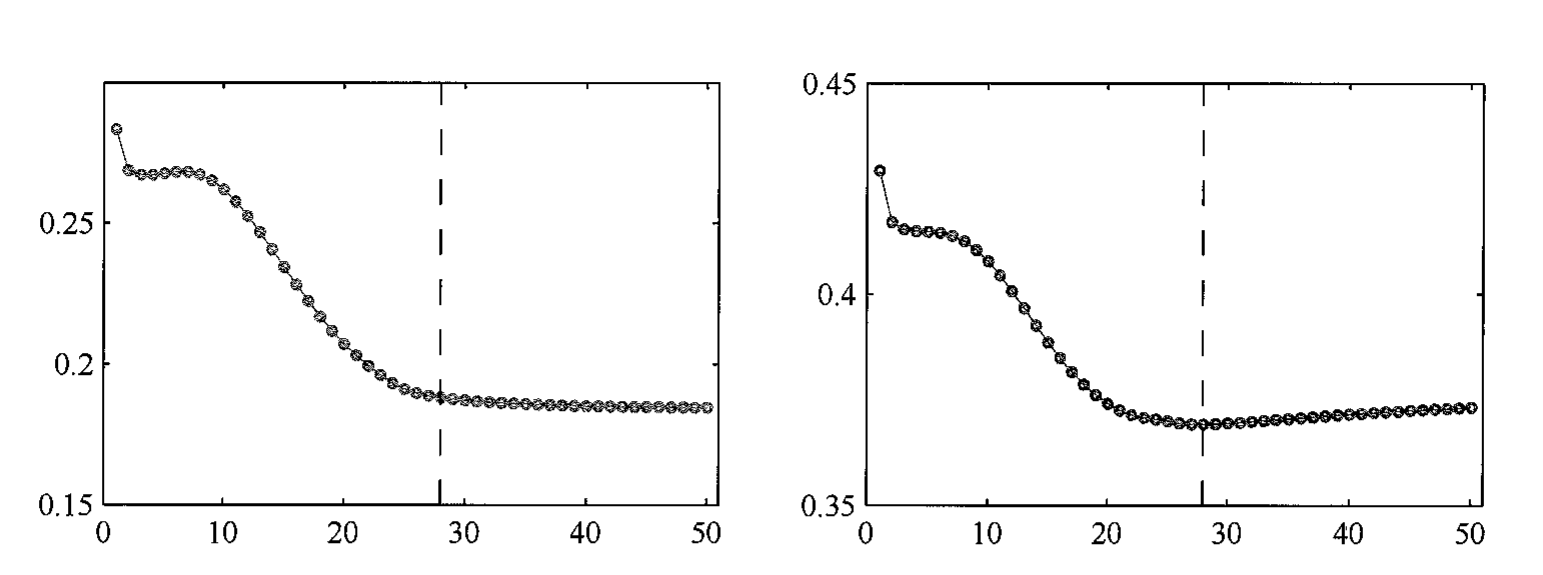
\includegraphics[width=0.95\textwidth]{ch09-fig9-7-learning-curves.png}
\caption{在正弦数据集上进行的典型训练过程中，训练误差（左）和验证误差（右）关于迭代次数的函数的示意图。为了达到最佳的泛化能力，应在垂直虚线所示的迭代轮次停止训练，此处对应验证误差的最小值}
\label{figure:ch09-学习曲线}
\end{figure}

学习曲线的这种现象有时可以从网络中有效参数数量的角度进行定性解释。这个数量开始时很少，然后在训练过程中增长，对应模型有效复杂度的稳定增加。在训练误差达到最小值之前，停止训练是限制网络有效复杂度的一种方法。

我们可以在二次误差函数上验证这一洞察，结果显示早停法与使用简单权重衰减项的正则化（Bishop，1995a）作用相似。\cref{figure:ch09-早停}对此做了说明，权重空间中的轴已经旋转以与 Hessian 矩阵的特征向量平行。如果在没有权重衰减的情况下（参见\cref{section:ch07-错误平面}），权重向量从原点开始，并在训练期间沿着局部负梯度向量的路径前进，那么权重向量将从最初与 $\boldsymbol{w}_{2}$ 轴平行，大约朝着 $\boldsymbol{w}^{*}$ 移动，最后向误差函数的最小值移动。这种移动方法遵循误差表面的形状，并且与 Hessian 矩阵的特征值有很大不同。因此，在 $\hat{\boldsymbol{w}}$ 附近的某个点停止训练类似于权重衰减。早停法和权重衰减之间的关系可以被量化（参见\cref{exercise:ch09-06}），从而显示出量 $\rho\tau$（其中 $\tau$ 是迭代次数，$\rho$ 是学习率）可以像正则化参数 $\lambda$ 的倒数一样发挥作用。因此，网络中有效参数的数量在训练期间会增长。

\begin{theorem}[早停与权重衰减的等价性]\label{theorem:ch09-早停等价}
设未正则化误差函数为
\begin{align*}
E(\boldsymbol{w})=E_{0}+\frac{1}{2}(\boldsymbol{w}-\boldsymbol{w}^{*})^{\mathsf T}\boldsymbol{H}(\boldsymbol{w}-\boldsymbol{w}^{*}),
\end{align*}
其中 $\boldsymbol{H}$ 对称正定，$\boldsymbol{w}^{*}$ 为最小值点。取初始值 $\boldsymbol{w}^{(0)}=\boldsymbol{0}$，并用学习率 $\rho>0$ 作梯度下降
\begin{align*}
\boldsymbol{w}^{(\tau)}=\boldsymbol{w}^{(\tau-1)}-\rho\nabla E(\boldsymbol{w}^{(\tau-1)}).
\end{align*}
则
\begin{align*}
\boldsymbol{w}^{(\tau)}=\bigl[\boldsymbol{I}-(\boldsymbol{I}-\rho\boldsymbol{H})^{\tau}\bigr]\boldsymbol{w}^{*}.
\end{align*}
若 $\{(\eta_{j},\boldsymbol{u}_{j})\}$ 是 $\boldsymbol{H}$ 的正交特征对，$w_{j}^{(\tau)}=\boldsymbol{u}_{j}^{\mathsf T}\boldsymbol{w}^{(\tau)}$、$w_{j}^{*}=\boldsymbol{u}_{j}^{\mathsf T}\boldsymbol{w}^{*}$，则
\begin{align*}
w_{j}^{(\tau)}=\bigl[1-(1-\rho\eta_{j})^{\tau}\bigr]w_{j}^{*}.
\end{align*}
进一步，设 $0<\rho\eta_{j}<1$ 对所有 $j$ 成立且 $\tau$ 充分大。则对 $\eta_{j}\gg(\rho\tau)^{-1}$ 的分量有 $w_{j}^{(\tau)}\approx w_{j}^{*}$，对 $\eta_{j}\ll(\rho\tau)^{-1}$ 的分量有 $|w_{j}^{(\tau)}|\ll|w_{j}^{*}|$。这正是权重衰减解
\begin{align*}
\boldsymbol{w}_{\lambda}=(\boldsymbol{H}+\lambda\boldsymbol{I})^{-1}\boldsymbol{H}\boldsymbol{w}^{*}
\end{align*}
在 $\lambda=(\rho\tau)^{-1}$ 处的逐分量行为。
\end{theorem}

\begin{proof}
（重构新增）令 $\boldsymbol{u}^{(\tau)}=\boldsymbol{w}^{(\tau)}-\boldsymbol{w}^{*}$。由 $\nabla E(\boldsymbol{w})=\boldsymbol{H}(\boldsymbol{w}-\boldsymbol{w}^{*})$，更新式变为
\begin{align*}
\boldsymbol{u}^{(\tau)}=\boldsymbol{u}^{(\tau-1)}-\rho\boldsymbol{H}\boldsymbol{u}^{(\tau-1)}=(\boldsymbol{I}-\rho\boldsymbol{H})\boldsymbol{u}^{(\tau-1)}.
\end{align*}
初始条件为 $\boldsymbol{u}^{(0)}=\boldsymbol{w}^{(0)}-\boldsymbol{w}^{*}=-\boldsymbol{w}^{*}$。递推得 $\boldsymbol{u}^{(\tau)}=-(\boldsymbol{I}-\rho\boldsymbol{H})^{\tau}\boldsymbol{w}^{*}$，故
\begin{align*}
\boldsymbol{w}^{(\tau)}=\boldsymbol{w}^{*}-(\boldsymbol{I}-\rho\boldsymbol{H})^{\tau}\boldsymbol{w}^{*}=\bigl[\boldsymbol{I}-(\boldsymbol{I}-\rho\boldsymbol{H})^{\tau}\bigr]\boldsymbol{w}^{*}.
\end{align*}
在特征基下，$\boldsymbol{H}^{\tau}\boldsymbol{u}_{j}=\eta_{j}^{\tau}\boldsymbol{u}_{j}$，且 $(\boldsymbol{I}-\rho\boldsymbol{H})^{\tau}\boldsymbol{u}_{j}=(1-\rho\eta_{j})^{\tau}\boldsymbol{u}_{j}$，故第 $j$ 个分量为 $w_{j}^{(\tau)}=[1-(1-\rho\eta_{j})^{\tau}]w_{j}^{*}$。当 $|1-\rho\eta_{j}|<1$ 即 $0<\rho\eta_{j}<2$ 时，$(\boldsymbol{I}-\rho\boldsymbol{H})^{\tau}\to\boldsymbol{0}$，从而 $\boldsymbol{w}^{(\tau)}\to\boldsymbol{w}^{*}$。

下面比较有限 $\tau$ 的行为。若 $\eta_{j}\gg(\rho\tau)^{-1}$，则 $\rho\eta_{j}\tau\gg1$，且
\begin{align*}
(1-\rho\eta_{j})^{\tau}\approx e^{-\rho\eta_{j}\tau}\approx0,
\end{align*}
故 $w_{j}^{(\tau)}\approx w_{j}^{*}$。若 $\eta_{j}\ll(\rho\tau)^{-1}$，则 $\rho\eta_{j}\tau\ll1$。由二项式展开
\begin{align*}
(1-\rho\eta_{j})^{\tau}=1-\rho\eta_{j}\tau+O\bigl((\rho\eta_{j}\tau)^{2}\bigr),
\end{align*}
故 $w_{j}^{(\tau)}\approx\rho\eta_{j}\tau\,w_{j}^{*}$，从而 $|w_{j}^{(\tau)}|\ll|w_{j}^{*}|$。另一方面，由\cref{theorem:ch09-L2闭式解}，权重衰减的第 $j$ 个分量为
\begin{align*}
w_{j}^{\lambda}=\frac{\eta_{j}}{\eta_{j}+\lambda}w_{j}^{*}.
\end{align*}
取 $\lambda=(\rho\tau)^{-1}$：当 $\eta_{j}\gg\lambda$ 时 $\frac{\eta_{j}}{\eta_{j}+\lambda}\approx1$，当 $\eta_{j}\ll\lambda$ 时 $\frac{\eta_{j}}{\eta_{j}+\lambda}\approx\frac{\eta_{j}}{\lambda}=\rho\eta_{j}\tau$。这与上面的两个渐近式逐一吻合。
\end{proof}

% SUPPLEMENT: parent=theorem:ch09-早停等价; kind=motivation; location=紧随其后的 remark（重构新增）
\begin{remark}（重构新增）\cref{theorem:ch09-早停等价}说明早停不是“另一种正则化”的类比，而是在二次误差、从原点出发、学习率足够小的条件下与权重衰减的精确对应：迭代次数 $\tau$ 扮演 $1/(\rho\lambda)$ 的角色，训练越久等价于 $\lambda$ 越小。由此可以解释\cref{figure:ch09-早停}：梯度下降的轨迹先沿 Hessian 大特征值方向快速下降，再沿小特征值方向缓慢前进；在 $\hat{\boldsymbol{w}}$ 处停止，相当于让小特征值方向的分量还来不及长大，这与权重衰减压制小曲率方向的效果一致。必须注意这个等价性的边界：它依赖二次误差、固定学习率、从原点初始化；对非线性网络只是局部近似，且学习率过大时 $|1-\rho\eta_{j}|<1$ 可能不成立，训练会发散而不是正则化。此外，早停的有效参数数随 $\tau$ 增长，这与 $\lambda$ 固定时有效参数数固定的情形不同：早停对应一条“随时间变化的正则化路径”。
\end{remark}

\begin{figure}[htbp]
\centering
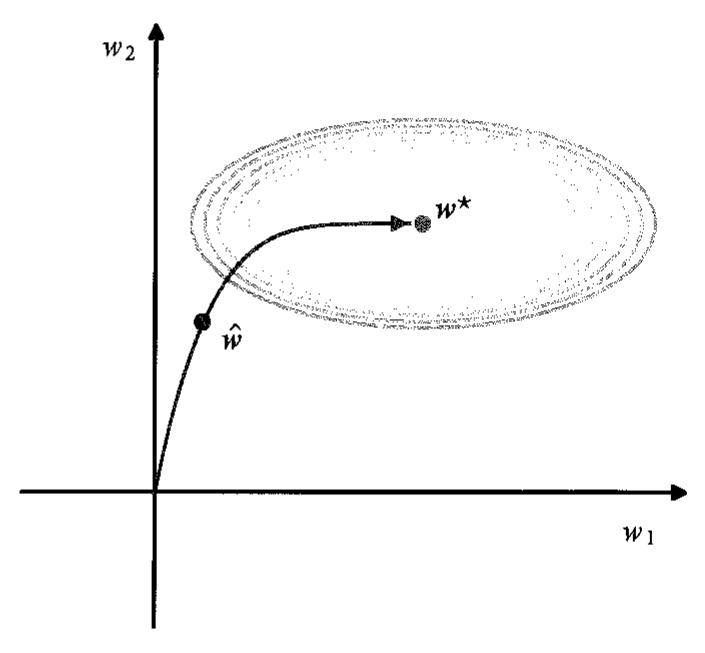
\includegraphics[width=0.52\textwidth]{ch09-fig9-8-early-stopping.png}
\caption{对于二次误差函数，早停法可以给出与权重衰减相似结果的示意图。椭圆显示了恒定误差的等值线，$\boldsymbol{w}^{*}$ 表示对应于未正则化误差函数最小值的最大似然解。如果权重向量从原点开始，并根据局部负梯度方向移动，那么权重向量将沿着图中所示的路径前进。通过与\cref{figure:ch09-权重衰减等值线}进行比较可以看出，提前停止训练后，就可以找到一个权重向量 $\hat{\boldsymbol{w}}$，从而发现这与使用简单的权重衰减正则化项，并训练到正则化误差最小时的结果类似}
\label{figure:ch09-早停}
\end{figure}

\subsection{双重下降}\label{subsection:ch09-双重下降}

偏差--方差权衡为可学习模型的泛化能力会随着模型参数数量的变化而变化提供了解释（参见\cref{section:ch04-偏差方差权衡}）。参数太少的模型会因为有限的表现能力（高偏差）而有较大的测试误差；随着参数数量的增加，可以预期测试误差会降低。然而，随着参数数量的进一步增加，由于过拟合（高方差），测试误差会再次上升。这引出了经典统计学中一个普遍的观念，即模型中参数的数量需要根据数据集的大小进行限制：对于给定的训练集，非常大的模型预期表现不佳。

然而，与这种预期相反，对于现代深度神经网络，即使参数数量远远超过对训练数据完美拟合所需，也可以表现出色（Zhang et al.，2016）。深度学习社区的普遍看法是，更大的模型表现会更好。虽然有时提前停止训练，但模型也可能被训练到零误差，并且在测试数据上表现良好。

这些看似矛盾的观点可以通过检查学习曲线和其他模型复杂度对泛化能力的图表来解释，这些图表揭示了一种称为\textbf{双重下降}（double descent）的更微妙的现象（Belkin et al.，2019）。\cref{figure:ch09-双重下降}显示了一个名为 ResNet18 的大型神经网络模型（He et al.，2015a）中，训练误差和测试误差与模型复杂度（由可学习参数的数量决定）的关系。该网络有 18 层参数，是在图像分类任务上进行训练的。通过改变控制每层中隐藏单元数量的“宽度参数”，网络中的权重和偏置数量可以变化。我们看到，与预期一致，训练误差随着模型复杂度的增加而单调减小。然而，测试误差最初下降，然后再次上升，最后再次下降。虽然训练误差已经达到零，但测试误差仍旧持续减小。

\begin{definition}[双重下降]\label{definition:ch09-双重下降}
设模型复杂度由参数数量或某个连续控制参数（如宽度、训练轮次、$1/\lambda$）度量。若测试误差作为复杂度的函数先下降、再上升、最后再次下降，即出现两个下降段与中间一个峰值，则称这一现象为\textbf{双重下降}（double descent）。第一个下降段对应经典的偏差--方差权衡，峰值出现在模型刚好能够插值训练数据的临界区域附近，第二个下降段对应过参数化区域。
\end{definition}

% SUPPLEMENT: parent=definition:ch09-双重下降; kind=motivation; location=紧随其后的 remark（重构新增）
\begin{remark}（重构新增）\cref{definition:ch09-双重下降}中的“双重”指的是测试误差曲线上有两个下降段，而不是两个峰值。峰值的位置称为插值阈值：在它左侧，模型欠参数化，增加容量主要降低偏差；在它右侧，模型可以零误差拟合训练集，继续增加容量反而使隐式正则化（如随机梯度下降的偏好）挑选出更平滑的插值解，测试误差重新下降。这个现象并不否定偏差--方差权衡，而是说明“参数数量”不是复杂度的好度量：在插值阈值附近，有效复杂度急剧变化，单看参数个数会得出错误结论。还要注意，双重下降的第二个下降段依赖优化算法与初始化；同样的过参数化模型若训练不充分，可能停留在峰值附近而表现很差。
\end{remark}

两种模型拟合模式之间的过渡大约发生在模型中参数的数量足够多以至于能够精确拟合训练数据时（Belkin et al.，2019）。Nakkiran 等人（2019）定义了模型有效复杂度为模型可以在上面达到零训练误差的最大训练集大小，因此当模型有效复杂度超过训练集中数据点的数量时，就会出现双重下降。

\begin{definition}[模型有效复杂度]\label{definition:ch09-模型有效复杂度}
对给定的模型族与训练算法，称该模型能够在其上达到零训练误差的最大训练集大小为模型的\textbf{有效复杂度}（effective complexity）（Nakkiran et al.，2019）。当有效复杂度超过当前训练集的数据点数时，模型处于插值区域。
\end{definition}

% SUPPLEMENT: parent=definition:ch09-模型有效复杂度; kind=motivation; location=紧随其后的 remark（重构新增）
\begin{remark}（重构新增）\cref{definition:ch09-模型有效复杂度}把复杂度从“参数个数”改为“能记住多少样本”，因而同时依赖模型族、优化算法与训练轮次。这个定义解释了为什么同一网络在不同训练轮次下表现出不同的有效复杂度：训练越久，模型能插值的样本越多，有效复杂度越高。它也给出双重下降的统一图景：无论横轴是参数个数、训练轮次还是 $1/\lambda$，只要该轴能推动模型越过插值阈值，就可能看到第二次下降。使用时要注意“零训练误差”是理想化条件；实际中应理解为低于某个很小的阈值，因此有效复杂度是一个依赖于阈值的量。
\end{remark}

\begin{figure}[htbp]
\centering
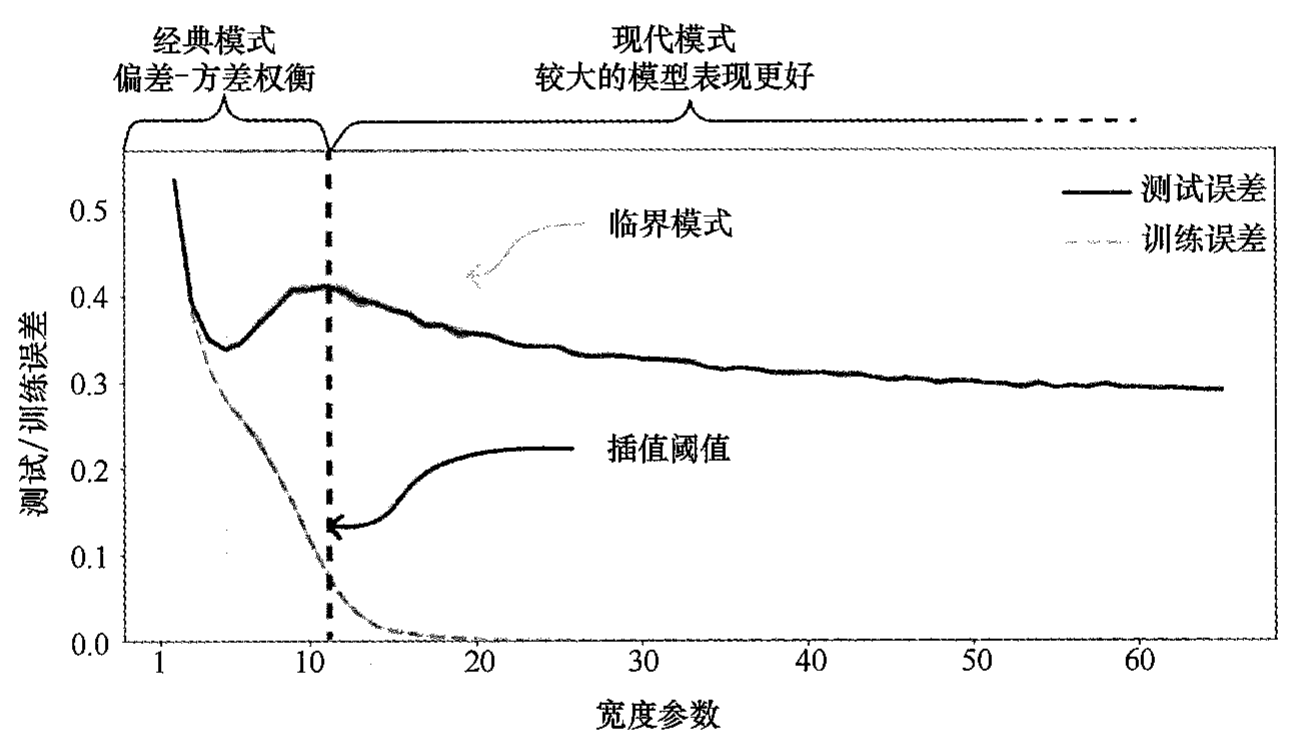
\includegraphics[width=0.82\textwidth]{ch09-fig9-9-double-descent.png}
\caption{一个名为 ResNet18 的大型神经网络模型在图像分类问题上训练误差和测试误差与模型复杂度的关系图。水平轴代表一个控制隐藏单元数量的超参数，因此也控制了网络中权重和偏置的总数。标记为“插值阈值”的竖直虚线表示原则上能够在训练集上达到零误差的模型复杂度水平［经 Nakkiran et al.（2019）授权使用］}
\label{figure:ch09-双重下降}
\end{figure}

这种令人惊讶的现象比通常从经典统计学的偏差--方差讨论中期望的现象更复杂，并呈现出两种不同的模型拟合模式，正如\cref{figure:ch09-双重下降}中所显示的，对应于小到中等复杂度的经典偏差--方差权衡，随后当我们进入大型模型的阶段时，测试误差进一步减小。

如\cref{figure:ch09-双重下降轮次}所示，如果使用早停法来控制模型复杂度，则可以看到类似的现象。增加训练轮次会增加模型有效复杂度，对于足够大的模型，我们将再一次观察到双重下降现象。

\begin{figure}[htbp]
\centering
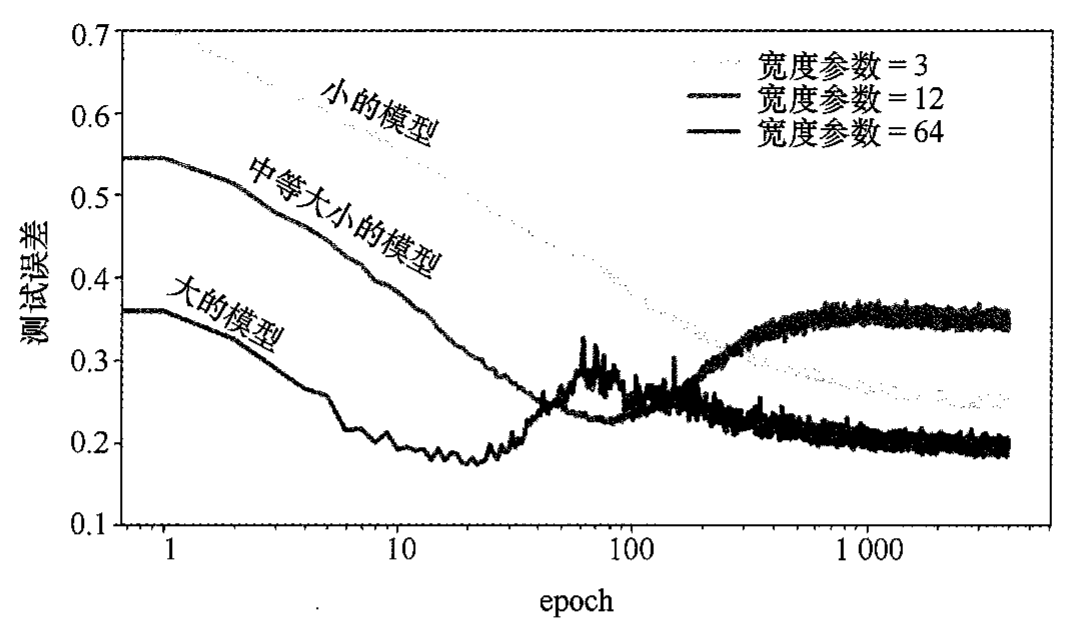
\includegraphics[width=0.82\textwidth]{ch09-fig9-10-double-descent-epoch.png}
\caption{ResNet18 模型的测试误差与梯度下降训练的训练轮次的关系图。模型有效复杂度随训练轮次的增加而增加，对于足够大的模型，可以观察到双重下降现象［经 Nakkiran et al.（2019）授权使用］}
\label{figure:ch09-双重下降轮次}
\end{figure}

当我们在误差函数中使用正则化项来控制模型复杂度时，可以得到类似的结果。在这里，一个训练到收敛的大型模型的测试误差显示出关于 $1/\lambda$（即正则化参数的倒数）的双重下降，因为较高的 $\lambda$ 对应于较低的模型复杂度（Yilmaz and Heckel，2022）。

双重下降的一个讽刺结果是，在某种情况下，增加训练集的大小实际上可能会降低性能，这与常识相悖，因为一般认为更多数据总是好事。对于\cref{figure:ch09-双重下降}中显示的处于临界阶段的模型，增加训练集的大小可以将插值阈值向右推，导致更高的测试误差。这在\cref{figure:ch09-双重下降样本量}中得到了确认，\cref{figure:ch09-双重下降样本量}显示了 Transformer 模型的测试误差关于输入空间维度（称为嵌入维度）的函数（参见\cref{chapter:ch12-Transformer与注意力机制}）。增加嵌入维度会增加模型中权重和偏置的数量，从而增加模型复杂度。我们看到，将训练集中数据点的数量从 4 000 增加到 18 000 可以得到整体上更低的曲线。然而，对于一定范围内的嵌入维度（对应处于临界复杂度阶段的模型），增加数据集的大小实际上可能会降低模型的泛化能力。

\begin{figure}[htbp]
\centering
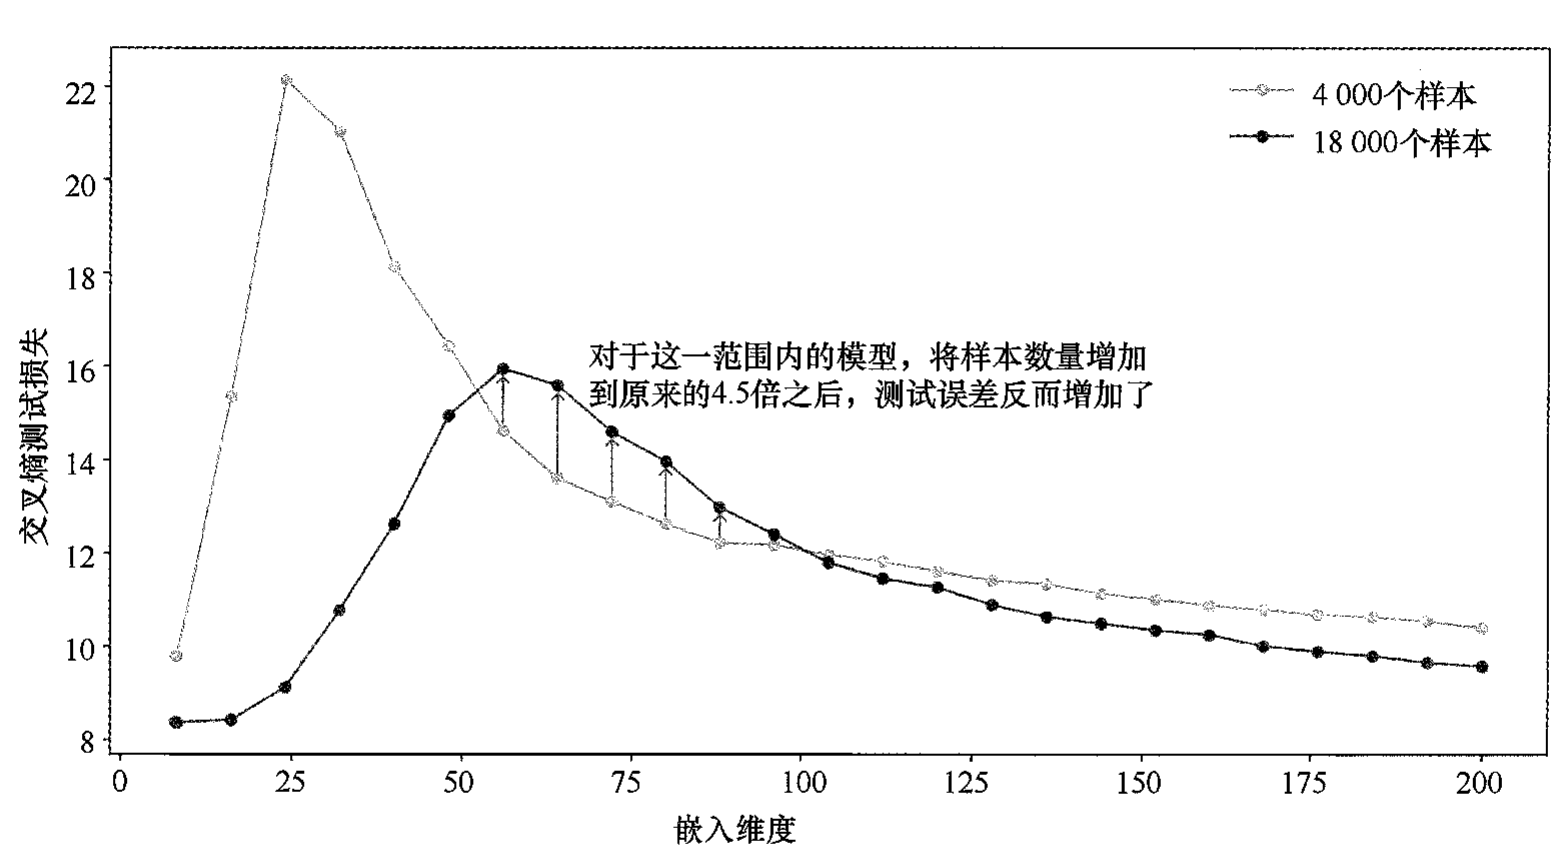
\includegraphics[width=0.92\textwidth]{ch09-fig9-11-transformer.png}
\caption{大型 Transformer 模型的测试误差与控制模型中参数数量的嵌入维度的关系图。将训练集的大小从 4 000 增加到 18 000 通常会使测试误差减小，但对于一些中等复杂度的模型，测试误差反而会增加，如垂直红色箭头所示［经 Nakkiran et al.（2019）授权使用］}
\label{figure:ch09-双重下降样本量}
\end{figure}

对于这样的模型，存在许多可能的解，包括那些过度拟合数据的解。因此，似乎是随机梯度下降引入的隐性偏见产生了良好的泛化能力。

\end{document}
